\section{Data and Methods}\label{sec:data_methods}


\subsection{Study scope and corridor design}\label{sec:scope}

The analysis targets deep-sea services between Northern Europe and Northeast Asia, 
where the choice of long-haul corridor has the largest implications for distance, 
time, fuel, and emissions. We select Rotterdam (51.95$^{\circ}$N, 4.14$^{\circ}$E) 
and Yokohama (35.45$^{\circ}$N, 139.65$^{\circ}$E) as the baseline 
origin--destination pair because it:
\begin{itemize}
  \item lies on a major Europe--Asia trade lane,
  \item is widely used in comparative corridor studies, and
  \item can be served via Suez, Cape of Good Hope, or the Northern Sea Route (NSR).
\end{itemize}
This ensures both operational relevance and comparability to earlier work, while 
magnifying routing-method effects over intercontinental distance.

We explicitly include three strategic maritime corridors:
\begin{enumerate}[label=(\roman*)]
    \item \textbf{Suez Canal Corridor (SUEZ)}: the established Europe--Asia trunk 
    route via the Mediterranean, Suez Canal, Red Sea, and Indian Ocean;
    \item \textbf{Cape of Good Hope Corridor (CAPE)}: a canal-independent fallback 
    via the Atlantic and Southern Indian Oceans, used during Suez and Red Sea 
    disruptions;
    \item \textbf{Northern Sea Route (NSR)}: the high-latitude Arctic corridor 
    along the Russian coast between the Barents Sea and Bering Strait.
\end{enumerate}

A global overview of these three corridors for the Rotterdam–Yokohama origin–destination pair is shown in Figure~\ref{fig:corridor_overview}.

For context, the direct great-circle distance between Rotterdam and Yokohama is about 5.1 k nm, i.e. substantially shorter than any of the corridorised routes considered here.

\begin{figure}[t]
  \centering
  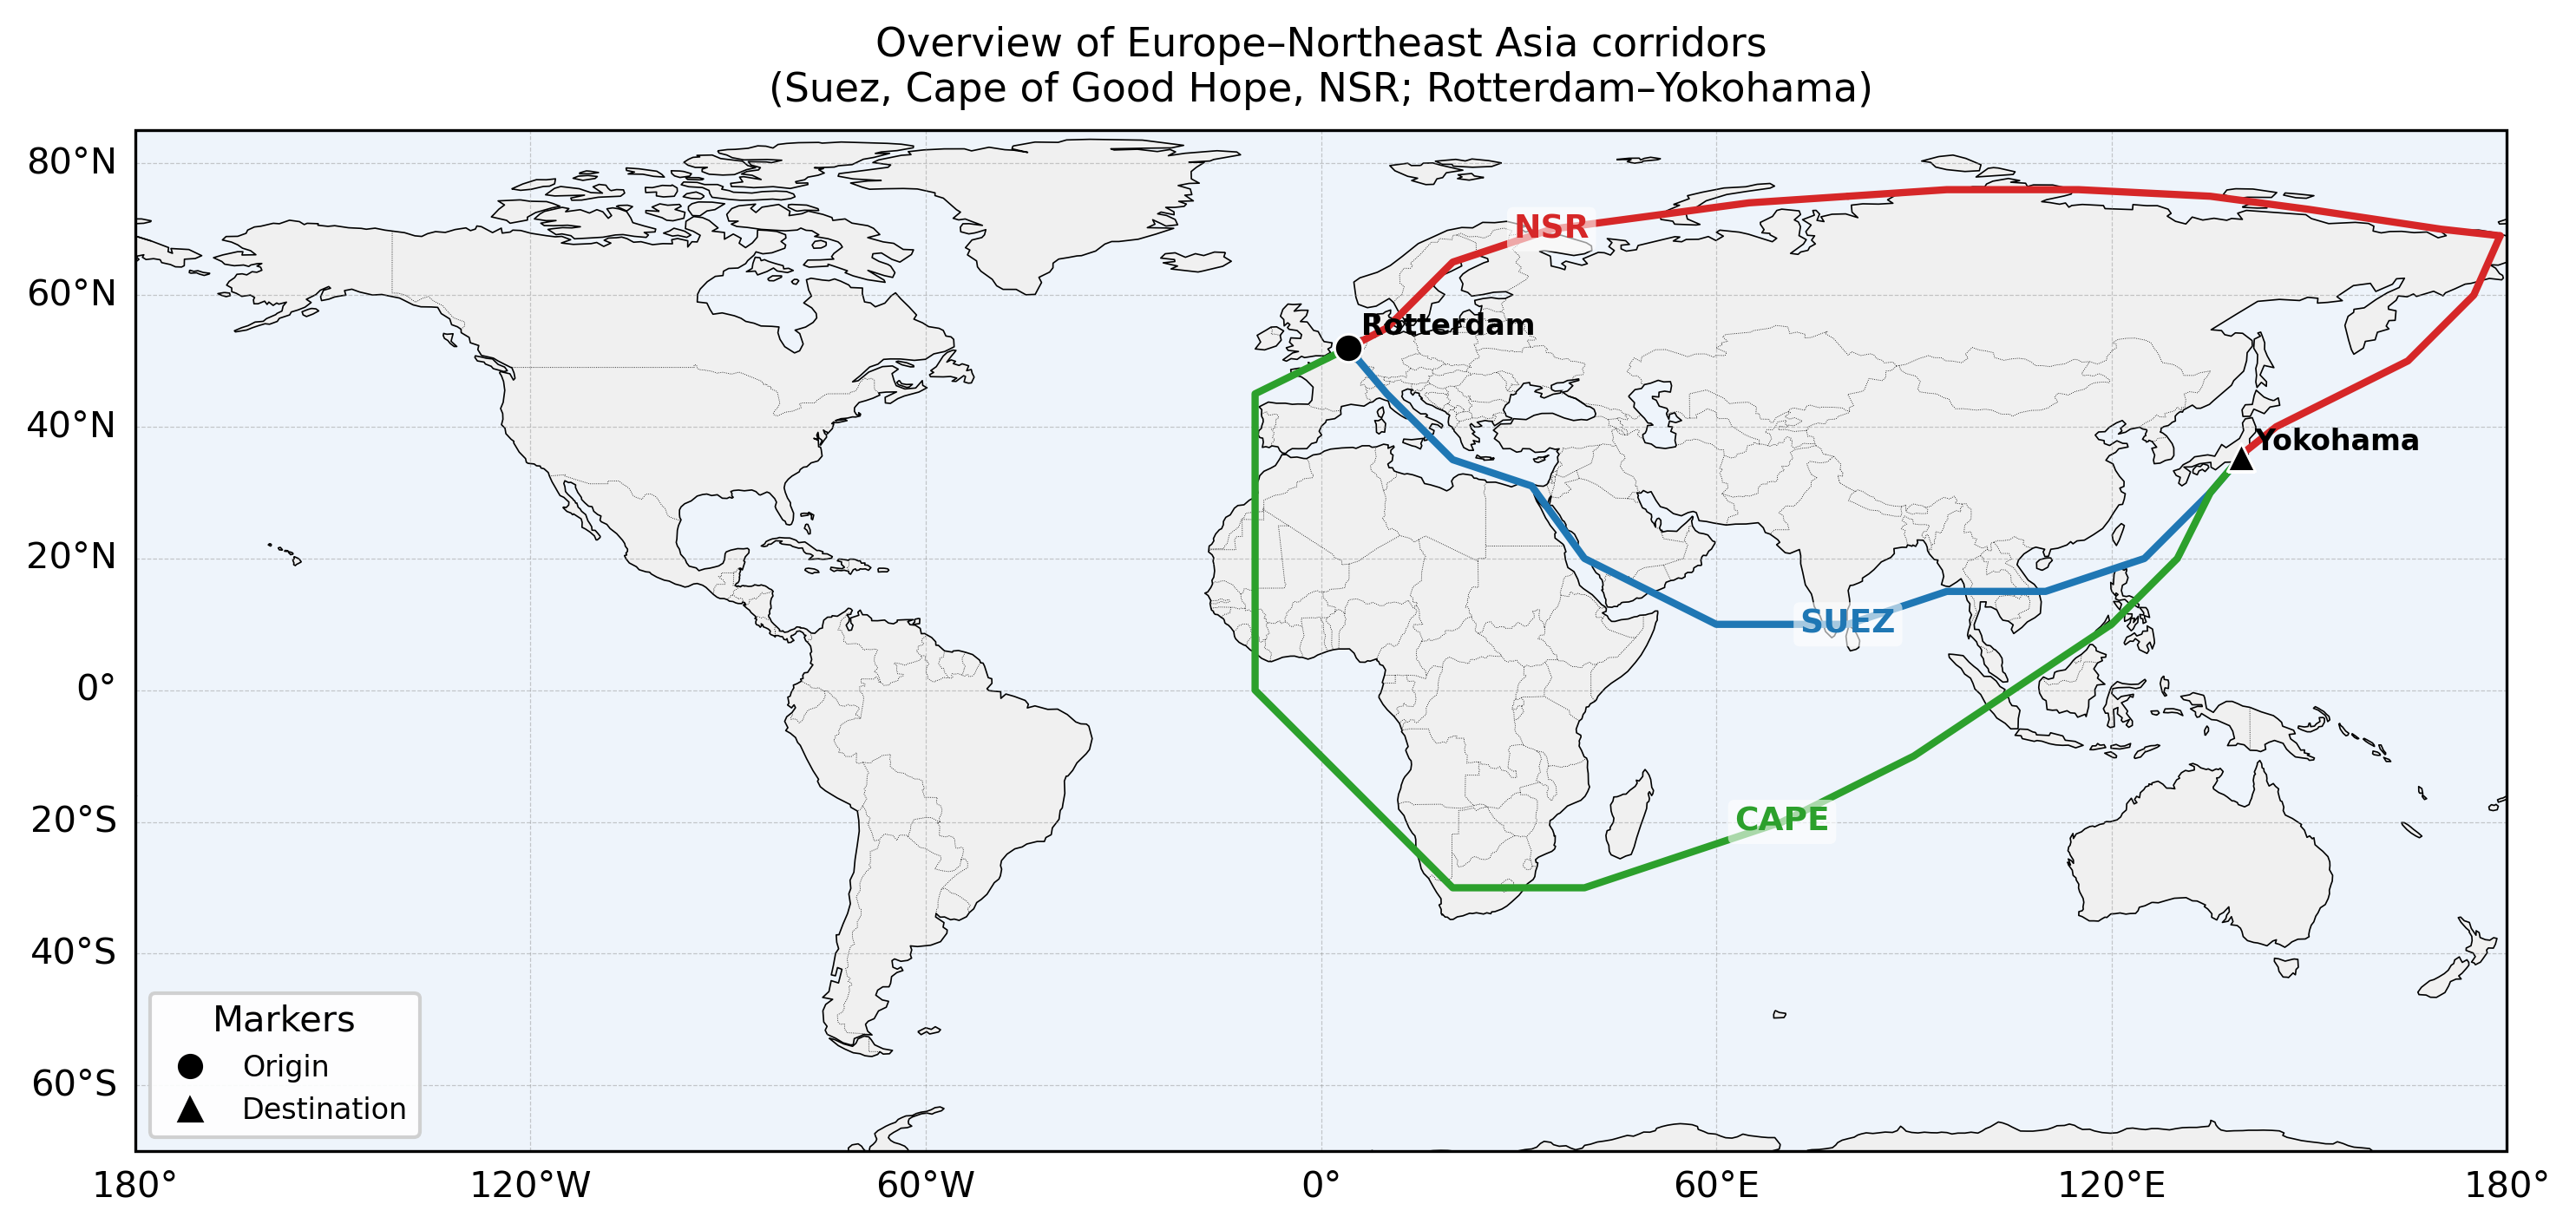
\includegraphics[width=\linewidth]{corridor_overview_world.png}
  \caption{Overview of the three Europe–Northeast Asia corridors considered in this study}
  \label{fig:corridor_overview}
\end{figure}


\FloatBarrier

We do not include the Panama Canal or the Northwest Passage. For the selected 
Northern Europe--Northeast Asia trade, Panama is not a competitive option, and 
the Northwest Passage remains operationally rare and heavily constrained. 
Including them would add complexity without materially changing the main corridor 
competition for this trade.

For each corridor we define three operational \emph{waypoint philosophies}:
\begin{enumerate}[label=(\alph*)]
  \item a \emph{service-guided} variant that loosely follows typical liner 
  schedules and gateway regions (major hubs and chokepoints);
  \item a \emph{bluewater-oriented} variant favouring longer open-ocean legs 
  where feasible; and
  \item a \emph{channel/coast-guided} variant that adheres more closely to 
  constrained straits and coastal guidance.
\end{enumerate}
These nine corridor--variant combinations bracket plausible operator routing 
styles without requiring detailed commercial schedules. Waypoints were defined manually based on contemporary sailing directions 
and publicly available track patterns, then verified via visual inspection 
on interactive charts to ensure they represent realistic chokepoints and 
gateway regions rather than arbitrary mid-ocean points. They allow us to assess whether the 
effects of routing representation (geometric vs.\ sea-only) persist across 
reasonable corridor geometries. 
The Macro waypoints and variant philosophies are summarized in Table~\ref{tab:waypoint_manifest}. 

\begin{table}[t]
  \centering
  \caption{Macro waypoint manifest and routing-variant philosophies for each corridor. 
  Variants correspond to (a) service-guided, (b) bluewater-oriented, and 
  (c) channel/coast-guided waypoint chains used to define corridor-specific GC and sea-only routes.}
  \label{tab:waypoint_manifest}
  \resizebox{\linewidth}{!}{%
    \begin{tabular}{lllrl}
\toprule
           scenario & corridor & philosophy &  n\_waypoints &                                    waypoints\_chain \\
\midrule
  CAPE\_VAR1\_service &     CAPE &       VAR1 &           10 & (52.0,4.1) → (36.0,-5.6) → (14.7,-17.5) → (-34.... \\
CAPE\_VAR2\_bluewater &     CAPE &       VAR2 &            9 & (52.0,4.1) → (30.0,-20.0) → (-10.0,-25.0) → (-3... \\
    CAPE\_VAR3\_coast &     CAPE &       VAR3 &           12 & (52.0,4.1) → (36.0,-5.6) → (5.0,-5.0) → (-20.0,... \\
   NSR\_VAR1\_service &      NSR &       VAR1 &            9 & (52.0,4.1) → (71.0,25.0) → (70.5,58.0) → (76.0,... \\
 NSR\_VAR2\_bluewater &      NSR &       VAR2 &            9 & (52.0,4.1) → (73.0,35.0) → (70.5,58.0) → (76.5,... \\
     NSR\_VAR3\_coast &      NSR &       VAR3 &            9 & (52.0,4.1) → (70.0,33.0) → (70.5,58.0) → (75.0,... \\
  SUEZ\_VAR1\_service &     SUEZ &       VAR1 &           10 & (52.0,4.1) → (50.5,1.0) → (36.0,-5.6) → (30.0,3... \\
SUEZ\_VAR2\_bluewater &     SUEZ &       VAR2 &           10 & (52.0,4.1) → (48.0,-10.0) → (36.0,-5.6) → (30.0... \\
    SUEZ\_VAR3\_coast &     SUEZ &       VAR3 &           13 & (52.0,4.1) → (50.5,1.0) → (36.0,-5.6) → (33.5,2... \\
\bottomrule
\end{tabular}

  }
\end{table}

\subsection{Routing representations: geometric GC vs.\ sea-only A*}\label{sec:routing}

We compare two routing representations for each corridor and waypoint variant.

\subsubsection{Great-circle baselines}\label{sec:gc}

Great-circle (GC) paths represent the geometric minimum distance between two 
points on a sphere. They are widely used in maritime and transport studies as 
distance benchmarks and as inputs to cost and emission models. However, raw GC 
arcs do not incorporate land--sea geometry, do not respect coastlines or 
chokepoints, and in principle may cross continental landmasses. In practice, 
GC-based corridor distances often reflect either (i) a single GC between origin 
and destination or (ii) a sum of GCs between a small set of corridor waypoints. 
In both cases, GC distances act as \emph{optimistic lower bounds} that idealise 
the Earth as a smooth sphere and abstract away navigational feasibility.

In this study, we construct for each corridor and waypoint variant a 
\emph{GC chain} connecting Rotterdam, the corridor-specific macro-waypoints, and 
Yokohama in sequence. These chains capture the geometric potential of each 
corridor and are representative of the kind of distances often invoked when the 
NSR is described as ``30--40\% shorter than Suez''.

\subsubsection{Sea-only routing with A*}\label{sec:astar}

To obtain physically feasible paths, we use the open-source \texttt{searoute} 
package \citep{searoute2022}, which implements a Dijkstra/A* shortest-path search on a global 
oceanic graph. Internally, \texttt{searoute} uses a regular latitude--longitude 
grid (approximately 0.5$^{\circ}$ resolution) whose nodes are constrained to 
water cells; coastlines and land are masked out when constructing the graph 
(as implemented in \texttt{searoute}'s default coastline mask). 
Edges connect neighbouring water nodes with weights proportional to 
great-circle segment length.

For each consecutive waypoint pair in a corridor's macro-waypoint chain, 
\texttt{searoute} is used to compute a sea-only shortest path. The resulting 
segments are concatenated to form a continuous sea-only polyline from Rotterdam 
to Yokohama. Every step of the search is constrained to water nodes; land and 
narrow straits act as hard constraints. This sea-only representation therefore captures corridor geometry, including 
high-latitude bends and mandatory chokepoints along each route (e.g.\ Bering 
Strait on the NSR, the Suez Canal, and the Cape of Good Hope), and provides an 
operationally meaningful approximation of feasible vessel trajectories. We verified algorithmic parity by confirming that A* and Dijkstra return identical shortest-path distances on the same sea graph.

The effective grid resolution (\mbox{$\approx 0.5^{\circ}$}) is chosen as a 
compromise between computational cost and geometric fidelity. At 
intercontinental scales, corridor-level differences in distance and time are 
insensitive to finer resolutions, whereas substantially coarser grids risk 
misrepresenting narrow passages or coastal stand-off. At 60$^{\circ}$N, a 
0.5$^{\circ}$ cell corresponds to roughly 15--30~nm spacing, adequate for corridor-scale benchmarking. 
Because our aim is to 
isolate \emph{routing-method effects} rather than resolve harbour approaches or 
traffic separation schemes (TSS), this resolution is sufficient.

Antimeridian crossings (near $\pm 180^{\circ}$ longitude) are handled through a 
combination of \texttt{searoute}'s internal graph representation and explicit 
dateline guards in post-processing, ensuring that polylines are continuous and 
free of wrap-around artefacts. Route geometries were validated by segment-length 
diagnostics to confirm no wrap-around jumps. Route polylines are subsequently interpolated 
to a uniform spacing (0.25$^{\circ}$) for consistent distance estimation.

\subsubsection{Rationale for comparing GC and A*}\label{sec:why_GC_Astar}

Comparing GC and A* isolates the effect of \emph{routing representation} itself: 
to what extent widely reported corridor advantages (e.g.\ ``NSR is 30--40\% 
shorter than Suez'') derive from geometric idealisations rather than navigable 
paths. GC chains bound the problem from below as idealised geometric minima. 
Sea-only A* routes represent the shortest navigable paths under static constraints, providing a conservative baseline prior to adding ice or weather costs.

Alternative graph-search or optimisation methods (e.g.\ Dijkstra on the same 
graph, dynamic programming, evolutionary heuristics, reinforcement learning) 
would return the same shortest path as A* under identical static constraints on 
a single-objective distance cost. Their added value lies in multi-objective or 
metocean-aware optimisation, which we deliberately reserve for subsequent work 
on dynamic voyage planning and environmental routing. The goal here is to 
cleanly separate the effect of moving from geometric GC representations to 
sea-only, coastline-respecting paths and to quantify how this transition 
propagates into distance, time, fuel, and CO$_2$ across the three corridors.

\subsection{From distance to time, fuel, and CO$_2$}\label{sec:energy_model}

For each scenario (corridor $\times$ waypoint philosophy $\times$ routing 
method), total route distance $D$ [nm] is computed as the sum of 
great-circle segment lengths along the GC chain or A* sea-only polyline.

Indicative voyage time is then obtained using corridor-specific average service 
speeds $U_{\text{corridor}}$ representative of current practice:
\begin{equation}
  T = \frac{D}{U_{\text{corridor}}},
\end{equation}
where $T$ is the sailing time. We do not optimise speeds; instead, we fix 
representative values to highlight how routing-method differences interact with 
realistic speed policies:
\begin{itemize}
    \item NSR: 12.5 kn (reflecting ice-class and high-latitude operational limits) \citep{shu2024_arctic_speed,li2024_nsr_speed_uncertainty};
    \item SUEZ: 14.5 kn (typical mainline container service under slow-steaming practice) \citep{bimco2024_container_outlook};
    \item CAPE: 14.0 kn (open-ocean service; conservative relative to Cape-rerouting averages) \citep{bimco2024_container_outlook}.
\end{itemize}
These values reflect corridor-typical slow-steaming practice and Arctic speed limits and are used to isolate routing-method effects rather than optimise operations \citep{bimco2024_container_outlook,shu2024_arctic_speed}.

Fuel consumption and CO$_2$ emissions are derived from voyage time using 
explicit main- and auxiliary-engine accounting. For the main engine, we assume a cubic speed--power relation and scale power from a reference operating point $(P_0,U_0)$:
\begin{equation}
  P_{\text{ME}} = P_0 \left(\frac{U}{U_0}\right)^3,
  \qquad 
  \dot{m}_{\text{ME}} = P_{\text{ME}} \cdot \mathrm{SFOC}_{\text{ME}},
\end{equation}
where $(P_0,U_0)$ is a reference condition (Table~\ref{tab:params}). 
SFOC values are converted from g\,kWh$^{-1}$ to t\,h$^{-1}$ using standard unit factors. 
Total main-engine fuel is $m_{\text{ME}} = \dot{m}_{\text{ME}} \, T$. 
Auxiliary-engine fuel is modelled as a constant power load over time,
$m_{\text{AUX}} = \dot{m}_{\text{AUX}} \, T$, capturing hotel and support loads 
during the voyage. The combined fuel consumption is then
\begin{equation}
  m_{\text{FUEL}} = m_{\text{ME}} + m_{\text{AUX}}.
\end{equation}
CO$_2$ emissions are computed using a standard emission factor 
$EF_{\text{CO2}}$ [t CO$_2$/t fuel]:
\begin{equation}
  m_{\text{CO2}} = m_{\text{FUEL}} \cdot EF_{\text{CO2}}.
\end{equation}

The cubic speed--power relation, constant SFOC, and CO$_2$ emission factor follow common practice in shipping 
emission inventories and IMO GHG studies \citep{emepeea_2019,imo_4th_ghg_2020,smith2014_third_ghg}. 
This level of detail is sufficient for isolating routing-method effects on 
voyage time, fuel, and CO$_2$; higher-fidelity resistance and engine 
models are reserved for subsequent work.

We intentionally retain a simple, transparent fuel and emission model so that 
the influence of routing representation on $T$, $m_{\text{FUEL}}$, and 
$m_{\text{CO2}}$ is fully traceable. Ship-specific resistance, 
weather-dependent added resistance, and speed-control strategies are left for 
follow-up work.

Representative parameter values (for a Panamax container vessel of 
approximately 50\,000--70\,000 DWT on conventional HFO) are summarised in 
Table~\ref{tab:params} and are consistent with standard 
practice in shipping emission inventories and IMO guideline assumptions 
\citep[e.g.][]{imo_4th_ghg_2020,emepeea_2019,smith2014_third_ghg}. 

A Panamax-class container vessel is used as a neutral baseline to convert voyage time into indicative fuel and CO$_2$. Absolute totals depend on ship size; however, under first-order scaling with common speed--power and SFOC assumptions, corridor rankings and relative routing-method deltas are expected to remain stable. Vessel-size sensitivity is examined in follow-on work. The parameter values are chosen to represent a generic Panamax vessel rather than a specific ship, so results reflect typical corridor-level behaviour instead of vessel-specific performance. The exact numerical values can be updated without changing the structure of the workflow.

\begin{table}[t]
  \centering
\caption{Assumed vessel, engine, and fuel parameters for the indicative 
time--fuel--CO$_2$ calculations (Panamax / small post-Panamax container 
vessel). Values can be adapted to other ship types without altering the methodology.}
  \label{tab:params}
  \begin{tabular}{lll}
    \toprule
    Symbol & Description & Value (example) \\
    \midrule
    $P_0$       & Reference main-engine power        & 35\,000 kW \\
    $U_0$       & Reference service speed            & 14.5 kn \\
    $\mathrm{SFOC}_\mathrm{ME}$ & Main engine SFOC        & 170 g\,kWh$^{-1}$ \\
    $P_\mathrm{AE}$      & Auxiliary power                & 2\,000 kW \\
    $\mathrm{SFOC}_\mathrm{AE}$ & Auxiliary SFOC          & 185 g\,kWh$^{-1}$ \\
    $EF_{\mathrm{CO_2}}$ & CO$_2$ factor (HFO)           & 3.114 t\,CO$_2$/t\,fuel \\
    $U_\mathrm{NSR}$     & Representative NSR speed       & 12.5 kn \\
    $U_\mathrm{SUEZ}$    & Representative Suez speed      & 14.5 kn \\
    $U_\mathrm{CAPE}$    & Representative Cape speed      & 14.0 kn \\
    \bottomrule
  \end{tabular}
\end{table}

All computations were performed in Python~3.11 using \texttt{pandas}, 
\texttt{geopy}, \texttt{shapely}, and \texttt{searoute}. Derived data tables were 
exported as CSV and \LaTeX{} tables, and visualised through static charts and 
interactive \texttt{folium} maps. 

\subsection{Scenario matrix and sensitivity tests}\label{sec:scenarios}

The primary scenario matrix consists of:
\begin{itemize}
  \item three corridors (SUEZ, CAPE, NSR);
  \item three waypoint philosophies per corridor (service-guided, 
  bluewater-oriented, channel/coast-guided);
  \item two routing representations (GC chain and A* sea-only); and
  \item corridor-specific average service speeds as in Table~\ref{tab:params}.
\end{itemize}
For each element in this matrix, we compute distance, indicative time, fuel, and 
CO$_2$ as described above.

To assess robustness, we perform several complementary sensitivity analyses:
\begin{enumerate}[label=(\alph*)]
  \item \textbf{Endpoint sensitivity:} repeating the analysis with an East Asia 
  endpoint in Busan instead of Yokohama to assess how NSR's relative advantage 
  changes for more northerly/westerly destinations.
  \item \textbf{Equal-speed comparisons:} repeating the time and fuel 
  calculations with a common service speed (14 kn) across all corridors to 
  isolate geometric and routing effects from speed policy.
\end{enumerate}

We deliberately exclude dynamic environmental and regulatory constraints (sea 
ice, winds, waves, currents, emission control areas, canal queues, ice 
pilotage/escort requirements) to maintain focus on routing-method effects. 
These factors will be layered onto the A* sea-only baseline in subsequent work 
on dynamic Arctic voyage planning.

\subsection{Computational workflow overview}

Figure~\ref{fig:pipeline} summarises the computational pipeline. 
Predefined macro-waypoints feed into GC and sea-only (A*) routing, from which 
distance--time--fuel--CO$_2$ metrics are derived under corridor-specific speeds. 
All intermediate outputs (routes, metrics, tables, and maps) are exported for 
reproducibility and further analysis.

\begin{figure}[t!]
 \centering
 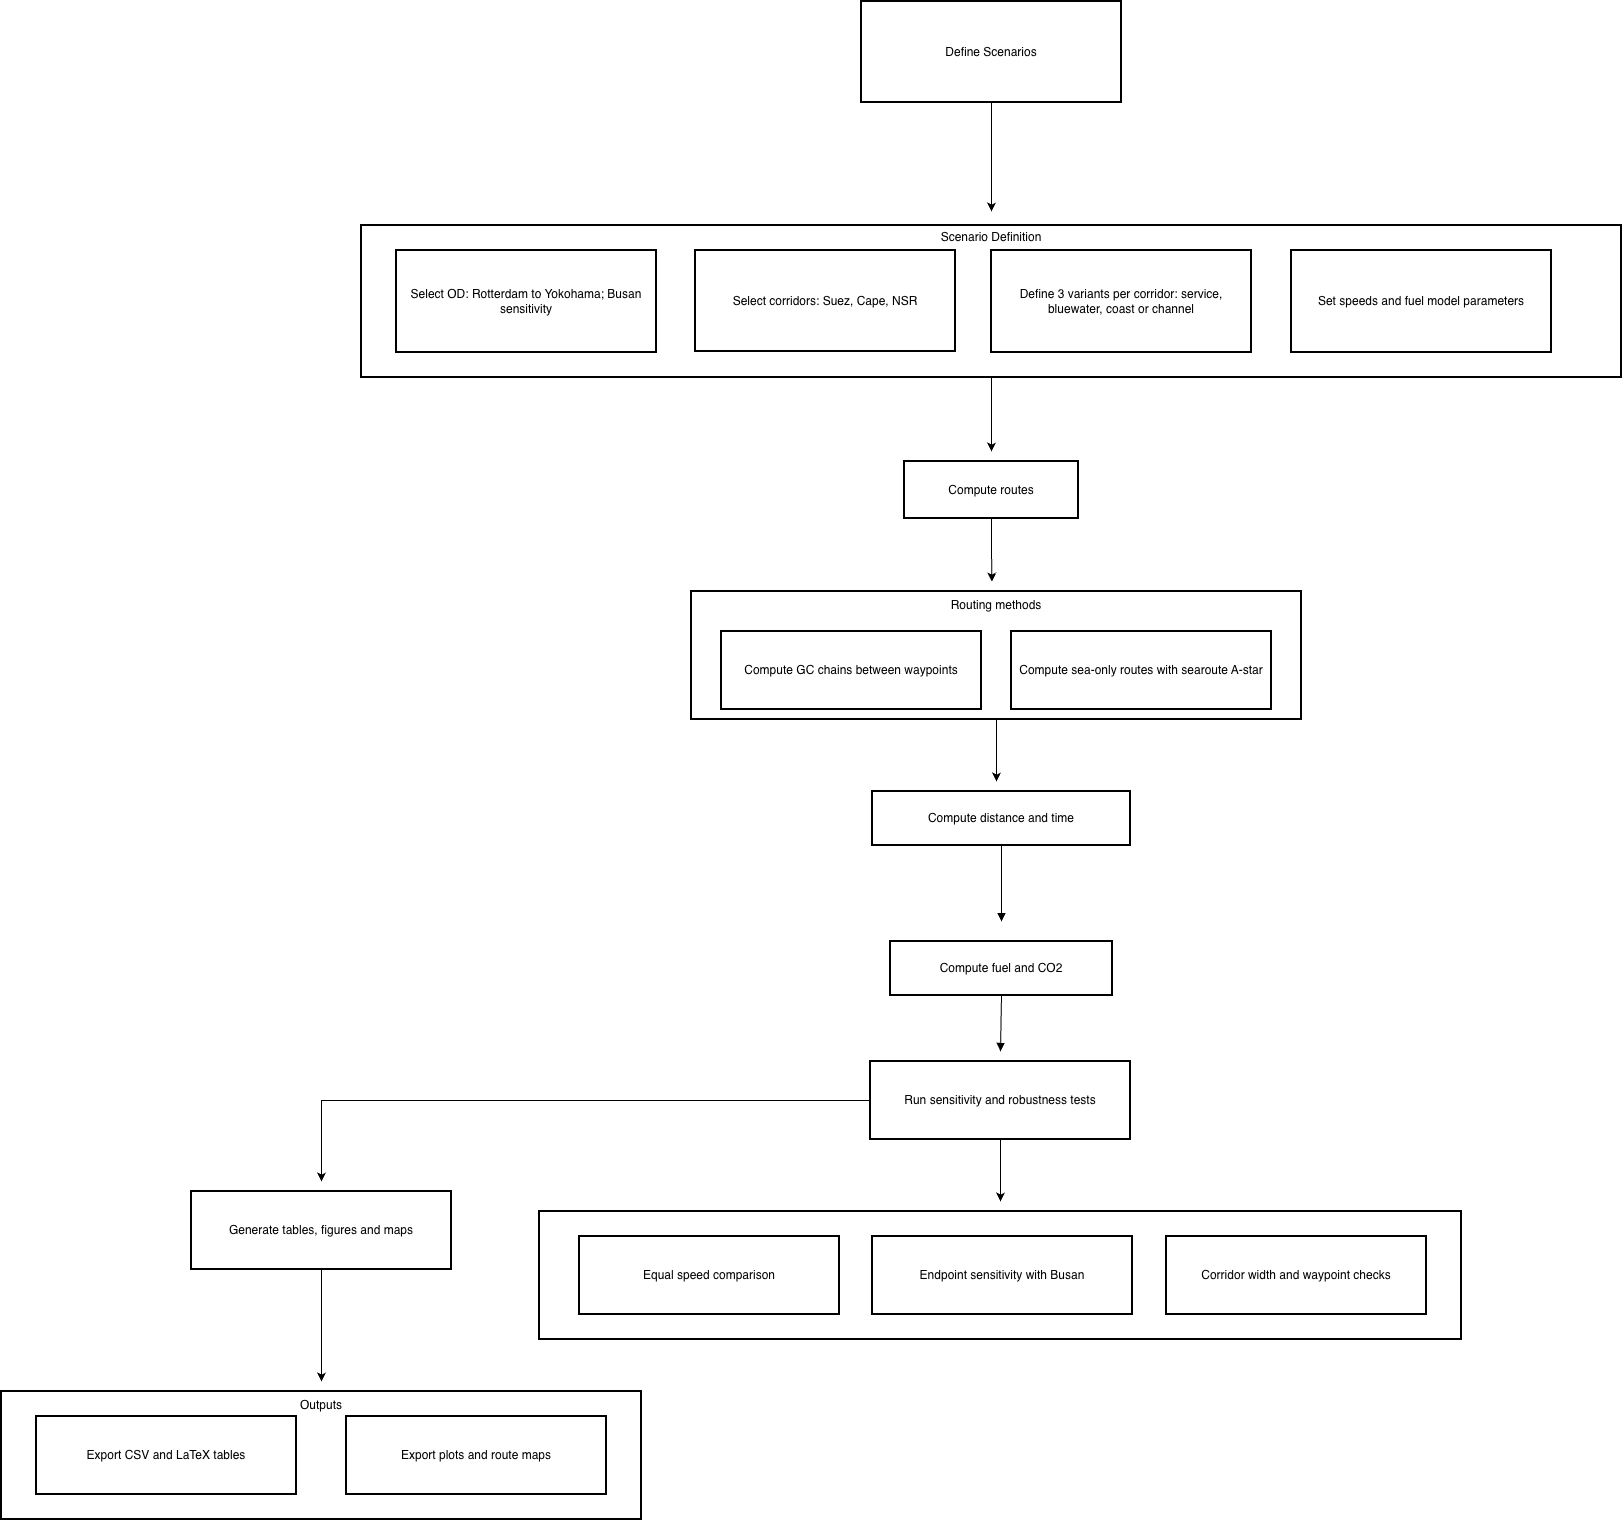
\includegraphics[width=0.9\linewidth]{pipeline.png}
 \caption{Overview of the methodological pipeline used to compute GC and sea-only routes, 
 derive time/fuel/CO$_2$ metrics, and generate reproducible tables and maps.}
 \label{fig:pipeline}
\end{figure}

\FloatBarrier
